\section{Background}
\label{sec:background}
Network on chip is an interconnect approach that helps different IPs and subsystems in a chip to communicate with each other in an efficient and scalable manner. 
In this approach each processing element (PE) is connected to a switch and multiple switches are interconnected to form a network.
A PE could be a processor core, a DSP core or an IP block.
The network infrastructure helps in routing data from one PE to another in the form of data packets. 
NoCs have found varying applications such as image and signal processing~\cite{Joshi2007}, multi-processor systems~\cite{Bertozzi2005}, virtual machine implementations~\cite{Mathias2006} etc.
Based on how the switches are interconnected, there are different NoC topologies such as mesh, torus, tree, ring, star, BFT etc. as shown in Fig.~\ref{fig:topologies}~\cite{ORTINOBON201624}.

\begin{figure}[t]
\centering
   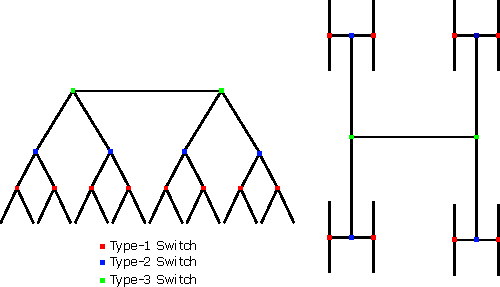
\includegraphics[width=\columnwidth]{Figures/HNoC.pdf}
   \caption{(a)A binary tree topology utilizing switches operating at different clock frequencies (b) The tree as an H-tree for better floorplanning on the FPGA}
   \label{fig:btree}
\end{figure}

In a mesh topology every switch, except the ones on the edges, is connected to 4 other neighboring switches.
A torus topology is similar to mesh but cyclic in nature.
In a binary tree, switches are arranged in a hierarchy.
Each switch has a parent node and two child nodes.
Unlike mesh and torus where each switch has a corresponding PE, in a tree topology only the switches at the bottom most level~(leaf nodes) are connected to PEs.

\begin{figure}[t]
\centering
   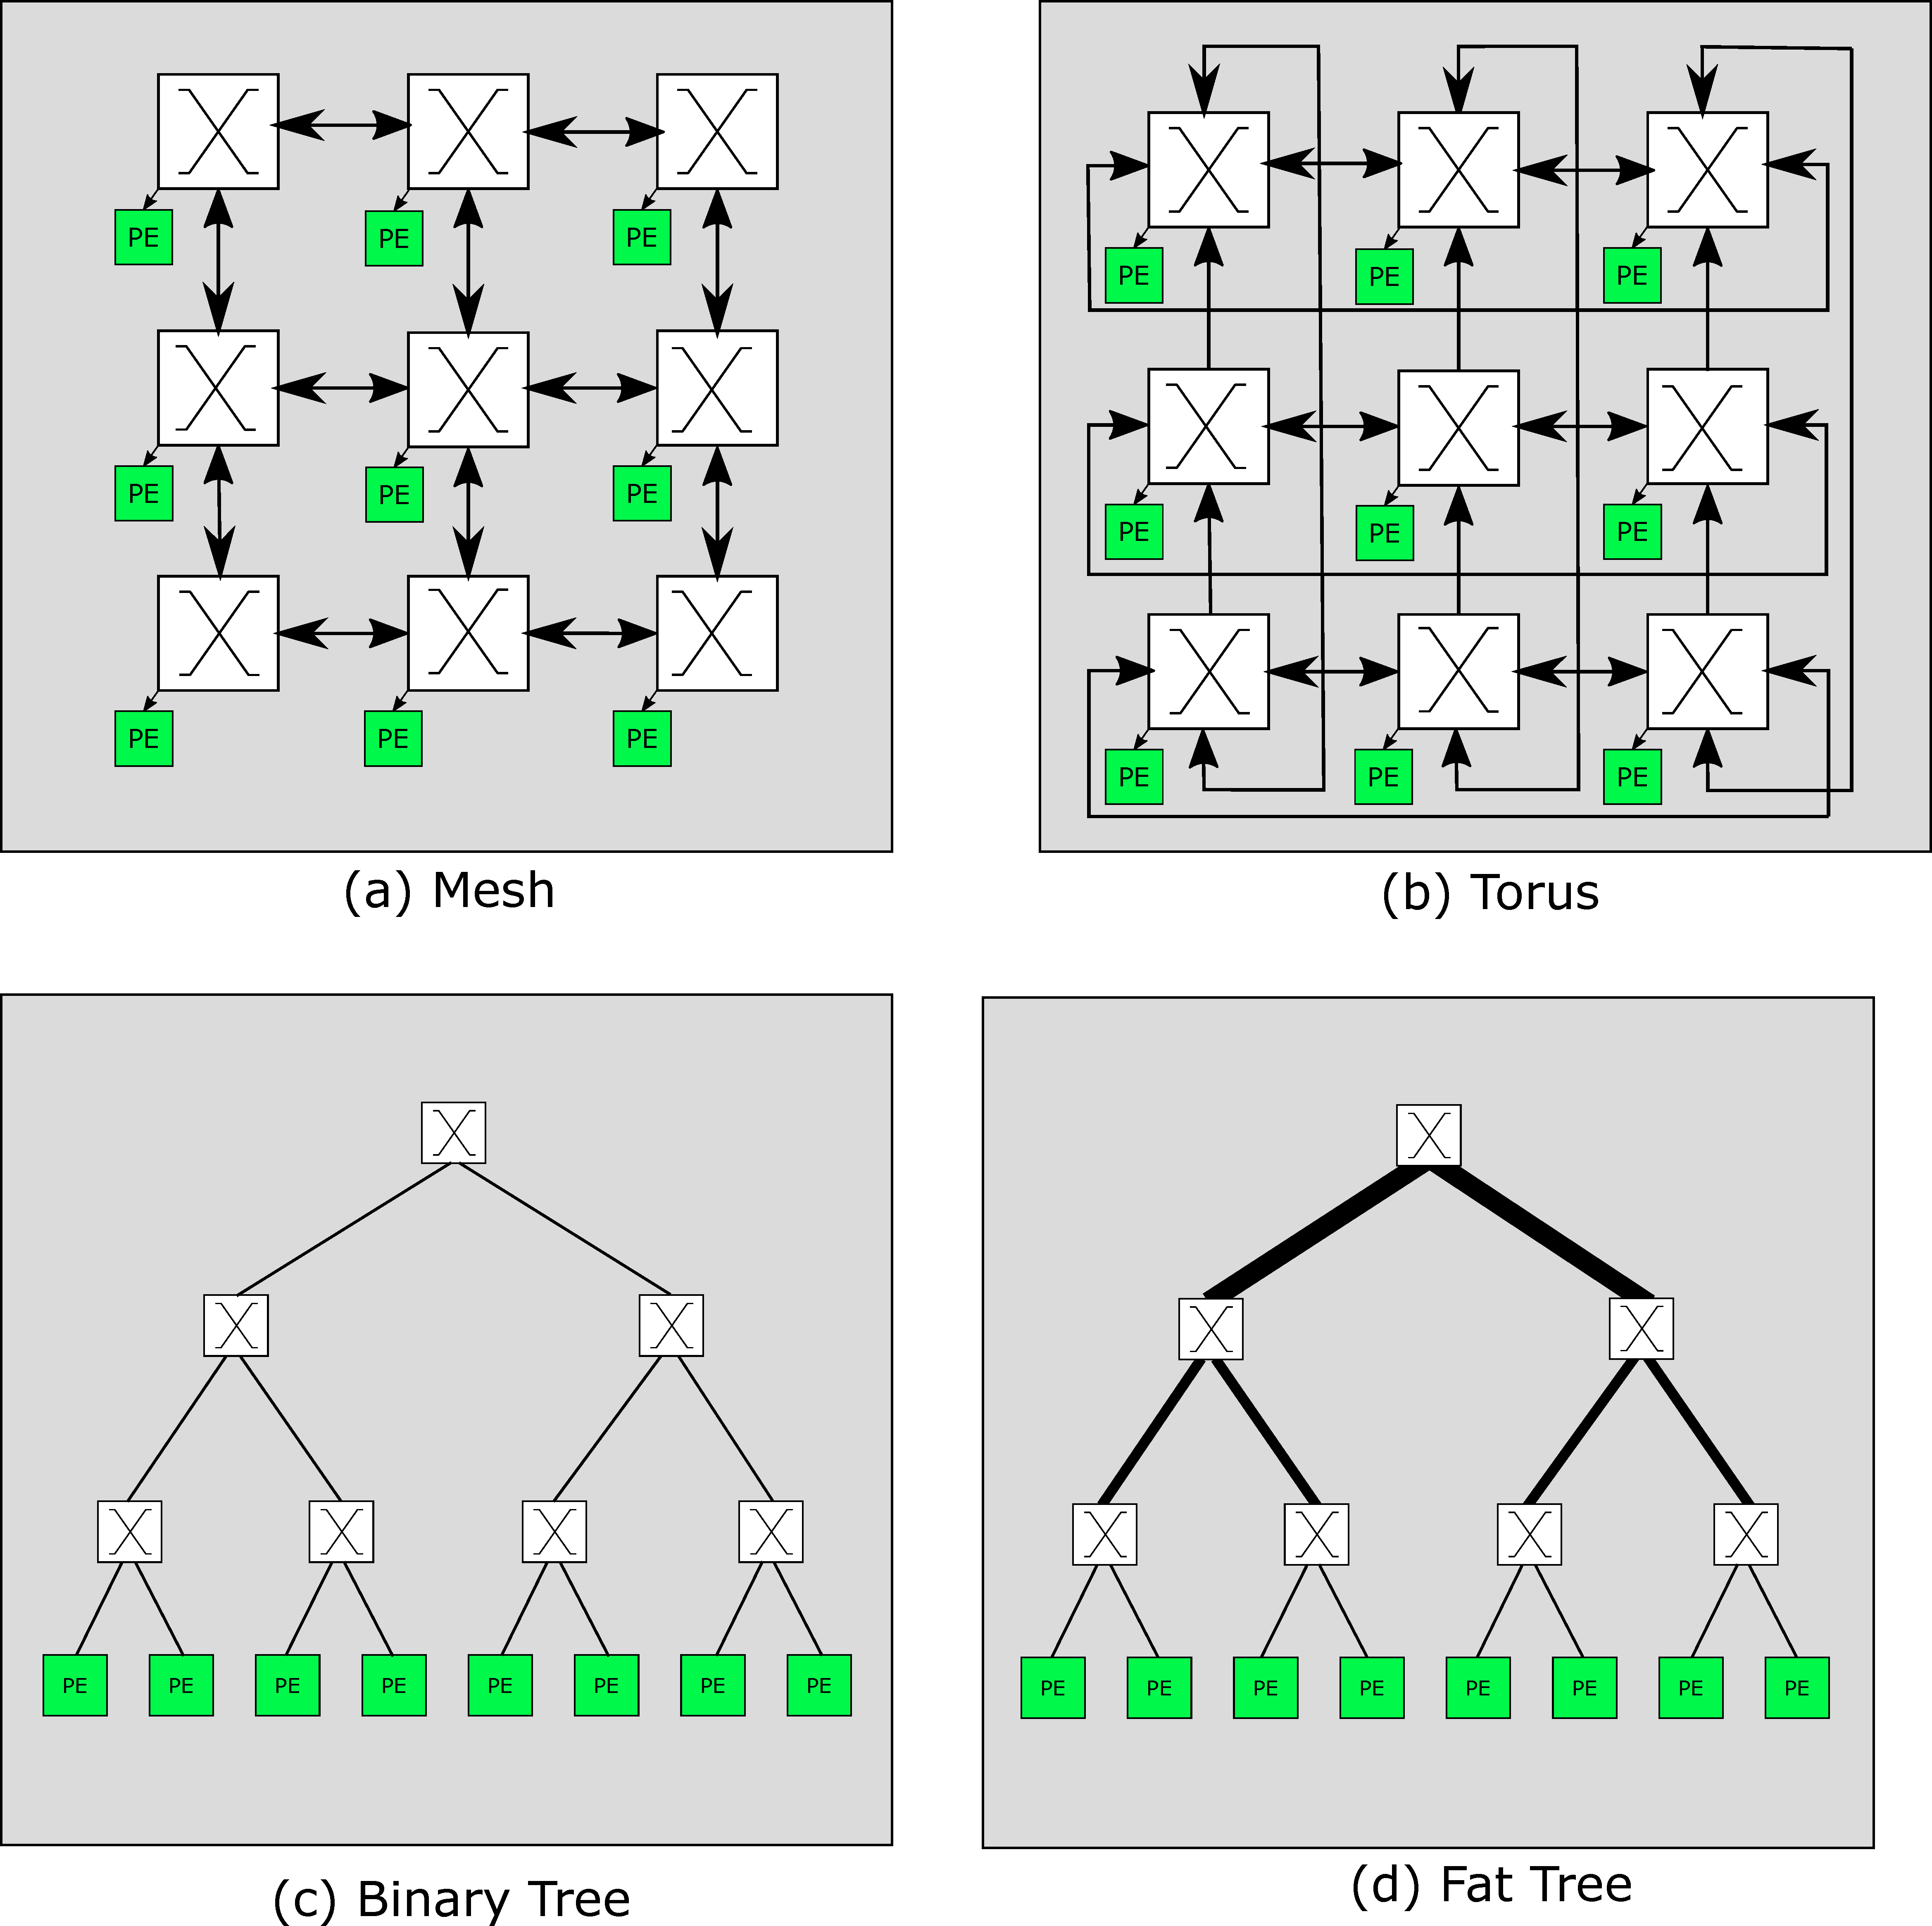
\includegraphics[width=\columnwidth]{Figures/topologies.pdf}
   \caption{Different NoC topologies}
   \label{fig:topologies}
\end{figure}

For interconnected networks, an important performance parameter is the bisection bandwidth~\cite{Wen-Chung2012}.
It is defined as the minimum bandwidth between two equal partitions of the network.
For a mesh topology, it is $\sqrt{n}*B$, where \emph{n} is the number of switches and \emph{B} is the bandwidth of a single link.
For torus, it is twice that of mesh but for a binary tree, it is only \emph{B}.
To address this issue, instead of using a single link between switches, more links can be used between them as we go higher in the tree hierarchy.
Such topology is called a fat tree~\cite{Leiserson1985,Ohring1995}. 
Although this will improve the bisection bandwidth, the switches in the upper hierarchy becomes more and more complex.
In this work we analyze whether using asynchronous switches with same link width can provide similar performance of fat trees while keeping relatively simpler switches.

\begin{figure}[t]
\centering
   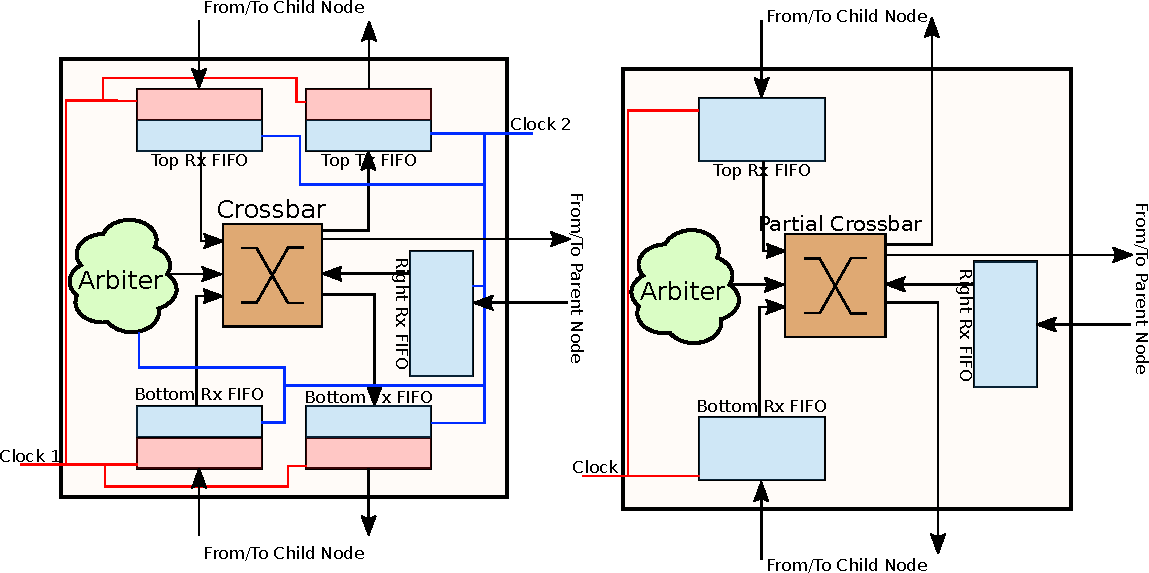
\includegraphics[width=\columnwidth]{Figures/switch1_2.pdf}
   \caption{Architecture of the different switches used in the AsyncBTree. (a) Type-1 switch used with the leaf nodes (PEs), with complete cross bar switch and asynchronous 
   FIFOs with receive and transmit interfaces (b) Type-2 switch used in intermediate nodes with partial crossbar switch and synchronous FIFOs (c) Type-3 switches used in intermediate
   switches with partial cross bar and asynchronous FIFOs with receive and transmit interfaces.}
   \label{fig:switchArch}
\end{figure}

There have been previous efforts to develop NoC architectures specifically targeting FPGAs.
CONNECT NoC generator is the most popular among them~\cite{papa_connect_fpga2012}.
CONNECT is inspired by the fact that FPGAs have a large routing infrastructure available compared to memory and logic elements and tries to exploit it. 
It supports different NoC topologies and uses a single stage pipeline mechanism  to minimize hardware and latency. 
It has low operating frequency and is still quite resource intensive as seen in Section~\ref{sec:result}. 
Split-merge is another NoC infrastructure developed at University of Pennsylvania~\cite{Huan2012}.
It tries to overcome the limited clock performance of CONNECT at the expense of few more resources.


To the best of our knowledge, there have been no previous efforts to implement asynchronous switch-based NoCs targeting FPGAs. 
In this work we give a quantitative analysis of the performance of asynchronous binary trees.
We compare their performance with traditional and fat trees as well as other popular FPGA NoCs.
The binary tree implementations are available as open-source for other researchers to verify and to improvise the designs.